\documentclass[a4paper]{article}
\usepackage[pdftex]{graphicx}
\usepackage[utf8]{inputenc}
\usepackage{enumerate}
\usepackage{href-ul}
\hypersetup{
	colorlinks=true,
	linkcolor=blue,
	urlcolor=blue}
\usepackage{siunitx}
\sisetup{locale=DE}
\usepackage{icomma}
\usepackage{amssymb}
\usepackage{geometry}
\geometry{a4paper, top=15mm, left=15mm, right=15mm, bottom=15mm,
	headsep=10mm, footskip=12mm}
\usepackage{tikz}
\usetikzlibrary{positioning}

\begin{document}
	
	\begin{enumerate}[1.]
		{\bf \item Basic electrical quantities}
		
		\begin{center}
			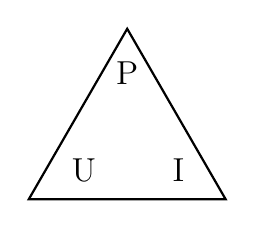
\begin{tikzpicture}[scale=1]
				% Dreieck mit Seitenlänge 2.5 cm
				\coordinate (U) at (0,0);
				\coordinate (I) at (2.5,0);
				\coordinate (P) at (1.25, {2.5*sqrt(3)/2});
				
				% Linien zeichnen
				\draw[thick] (U) -- (I) -- (P) -- cycle;
				
				% Beschriftung innerhalb
				\node[above=0.1cm of U, xshift=0.7cm] {\large U};
				\node[above=0.1cm of I, xshift=-0.6cm] {\large I};
				\node[below=0.3cm of P] {\large P};
			\end{tikzpicture}
			\hspace{3 cm}
			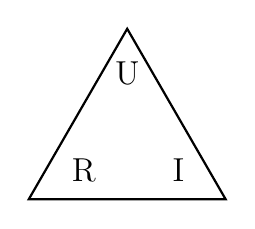
\begin{tikzpicture}[scale=1]
				% Dreieck mit Seitenlänge 2.5 cm
				\coordinate (R) at (0,0);
				\coordinate (I) at (2.5,0);
				\coordinate (U) at (1.25, {2.5*sqrt(3)/2});
				
				% Linien zeichnen
				\draw[thick] (R) -- (I) -- (U) -- cycle;
				
				% Beschriftung innerhalb
				\node[above=0.1cm of R, xshift=0.7cm] {\large R};
				\node[above=0.1cm of I, xshift=-0.6cm] {\large I};
				\node[below=0.3cm of U] {\large U};
			\end{tikzpicture}
		\end{center}
		
		\renewcommand{\arraystretch}{2}
		\begin{tabular}{|p{0.5 cm}|p{1.7 cm}|p{1.7 cm}|p{1.7 cm}|p{1.7 cm}|p{1.7 cm}|p{1.7 cm}|p {1.7 cm}|p{1.7 cm}|}
			\hline
			& Water cooker & LED & Electric car & Notebook & Router & Hydro\-electric power station & Energy saving lamp & Thun\-derstorm Lightning\\
			\hline
			U & 230 V & & & 20 V & 12 V & & 230 V & $\SI{1e8}{\volt}$\\
			\hline
			I & & 20 mA & 123 A & 3.25 A & & & & $\SI{1e5}{\ampere}$\\
			\hline
			P & 1200 W & & 80 kW & & & 20 MW & 7 W & \\
			\hline
			R & &$\SI{125}{\ohm}$& & & $\SI{3.6}{\ohm}$& $\SI{0.6}{\kilo\ohm}$& & \\
			\hline
		\end{tabular}
		
		{\bf \item Transformer}
		
		\renewcommand{\arraystretch}{2}
		\begin{tabular}{|p{2 cm}|p{2 cm}|p{2 cm}|p{2 cm}|p{2 cm}|p{2 cm}|p{2 cm}|}
			\hline
			& $U_p$ & $U_s$ & $N_p$ & $N_s$ & $I_p$ & $I_s$ \\
			\hline
			Power supply & 230 V & 12 V & 500 & & 0.12 A & \\
			\hline
			Welding machine & & 50 V & 610 & 80 & & 160 A \\
			\hline
			High voltage transformer & & 380 kV & 12 & & 500 A & 20 A \\
			\hline
		\end{tabular}
		
		{\bf \item Current and Charge}
		\begin{enumerate}[a)]
			\item A charger supplies the current $I=\SI{2}{\ampere}$. How long does it take for a battery with a capacity of $\SI{4000}{\milli\ampere\hour}$ to be fully charged?
			\item The same battery supplies a smartphone with energy for 48 hours. What is the average power consumption?
			\item A gold cap (small accumulator) supplies a bicycle rear light LED with a current of 20 mA for 12 minutes. What is the capacity in (mAh)?
			\item A small electric vehicle can run for one hour with 6.0 kW of power. What is the battery capacity in Ah if the operating voltage is 60 V?
		\end{enumerate}
		
		
	\end{enumerate}
	\fbox{
		\begin{minipage}{0.5\textwidth}
			For the solution, please \href{https://www.okuyakl.de/phys/p8puiL085/le085.pdf}{click here} or scan the QR code.\\
			Additional worksheets are available at
			
			\href{http://www.okuyakl.com}{www.okuyakl.com}
		\end{minipage}
		\hfill
		\begin{minipage}{0.4\textwidth}
			\includegraphics[width=1.5 cm]{../../viecher/zwe03}
			\includegraphics[width=3 cm]{qre085}
			\includegraphics[width=2 cm]{../../viecher/afanticon1}
			
	\end{minipage}}
\end{document}